\clearpage
\section{Monte Carlo Results}
\suppressfloats[t]

\subsection{Instrument Relevance and Point Estimation}

Table~\ref{tab:strength-calibration} establishes that the four values of $\kappa$ produce clearly ordered excluded-instrument relevance settings, using the first-stage $F$-statistic and partial $R^2$ as descriptive diagnostics.

\begin{table}[tbp]
  \caption{Instrument-strength calibration}
  \label{tab:strength-calibration}
  \begin{booktabs}{
    colspec = {Q[c] Q[c] Q[r] Q[c] Q[r] Q[c]},
    row{1} = {font = \bfseries}
  }
$n$ & $\kappa$ & Median $F$ & $F$: p10--p90 & Median partial $R^2$ & Partial $R^2$: p10--p90 \\
500 & 1.00 & 101.17 & 85.93--126.68 & 0.294 & 0.261--0.342 \\
500 & 0.50 & 18.71 & 11.99--27.95 & 0.071 & 0.047--0.103 \\
500 & 0.25 & 4.74 & 1.74--8.65 & 0.019 & 0.007--0.034 \\
500 & 0.10 & 1.22 & 0.24--3.65 & 0.005 & 0.001--0.015 \\
1000 & 1.00 & 212.82 & 185.34--239.50 & 0.301 & 0.273--0.327 \\
1000 & 0.50 & 38.65 & 30.13--53.60 & 0.073 & 0.058--0.098 \\
1000 & 0.25 & 9.85 & 5.34--16.15 & 0.020 & 0.011--0.032 \\
1000 & 0.10 & 2.04 & 0.38--5.42 & 0.004 & 0.001--0.011 \\
  \end{booktabs}
  \begin{tablenotes}[Note]
    Descriptive Monte Carlo strength diagnostics from the preserved 100-replication calibration. The reported dispersion ranges are the 10th and 90th percentiles. These statistics are not formal weak-instrument classification thresholds.
  \end{tablenotes}
\end{table}


Both diagnostics fall strongly as $\kappa$ decreases. For $n=500$, the median $F$-statistic falls from $101.17$ at $\kappa=1$ to $18.71$ at $\kappa=0.50$ and $1.22$ at $\kappa=0.10$; the corresponding endpoints for $n=1000$ are $212.82$ and $2.04$. Partial $R^2$ is comparatively stable across sample sizes, whereas $F$ increases with $n$. The design therefore varies the instruments' explanatory contribution while sample size affects the amount of information available. These diagnostics describe relative relevance within the experiment; they are not quantile-specific weak-IV thresholds.

Table~\ref{tab:main-performance} is the central finite-sample performance table. It reports Bias, MAE, RMSE, Coverage, and the median accepted-set measure for $n=1000$, $\tau\in\{0.10,0.50,0.90\}$, all four $\kappa$ values, and Oracle-GMM, Full-GMM, and DML-IVQR-BC.

% Prepared from frozen reporting CSVs; not yet inserted into Results.
\begin{table}[p]
  \small
  \caption{Main finite-sample performance at $n=1000$}
  \label{tab:main-performance}
  \begin{booktabs}{
    colspec = {Q[c] Q[c] X[l] Q[r] Q[r] Q[r] Q[r] Q[r]},
    colsep = 2pt,
    rowsep = 0pt,
    row{1} = {font = \bfseries},
    hline{14,26} = {\lightrulewidth, solid}
  }
$\tau$ & $\kappa$ & Estimator & Bias & MAE & RMSE & Coverage & {Median\\accepted-set\\measure} \\
\SetCell[r=12]{c} 0.10 & \SetCell[r=3]{c} 1.00 & Oracle-GMM & -0.054 & 0.093 & 0.121 & 0.860 & 0.400 \\
 &  & Full-GMM & -0.329 & 0.337 & 0.387 & 0.502 & 0.800 \\
 &  & DML-IVQR & -0.005 & 0.117 & 0.150 & 0.968 & 0.600 \\
 & \SetCell[r=3]{c} 0.50 & Oracle-GMM & -0.101 & 0.194 & 0.287 & 0.926 & 1.000 \\
 &  & Full-GMM & -0.407 & 0.465 & 0.630 & 0.804 & 1.900 \\
 &  & DML-IVQR & -0.159 & 0.306 & 0.482 & 0.948 & 2.225 \\
 & \SetCell[r=3]{c} 0.25 & Oracle-GMM & -0.384 & 0.566 & 0.934 & 0.930 & 3.450 \\
 &  & Full-GMM & -0.773 & 0.914 & 1.242 & 0.932 & 3.500 \\
 &  & DML-IVQR & -0.681 & 0.844 & 1.229 & 0.950 & 3.750 \\
 & \SetCell[r=3]{c} 0.10 & Oracle-GMM & -0.747 & 0.975 & 1.376 & 0.946 & 4.000 \\
 &  & Full-GMM & -1.074 & 1.251 & 1.582 & 0.942 & 3.900 \\
 &  & DML-IVQR & -0.932 & 1.146 & 1.514 & 0.936 & 4.000 \\
\SetCell[r=12]{c} 0.50 & \SetCell[r=3]{c} 1.00 & Oracle-GMM & 0.007 & 0.047 & 0.072 & 0.872 & 0.200 \\
 &  & Full-GMM & 0.007 & 0.072 & 0.100 & 0.896 & 0.400 \\
 &  & DML-IVQR & 0.070 & 0.079 & 0.104 & 0.776 & 0.300 \\
 & \SetCell[r=3]{c} 0.50 & Oracle-GMM & 0.015 & 0.093 & 0.134 & 0.936 & 0.500 \\
 &  & Full-GMM & 0.014 & 0.151 & 0.199 & 0.946 & 0.800 \\
 &  & DML-IVQR & 0.059 & 0.119 & 0.160 & 0.918 & 0.600 \\
 & \SetCell[r=3]{c} 0.25 & Oracle-GMM & 0.045 & 0.281 & 0.431 & 0.946 & 1.900 \\
 &  & Full-GMM & 0.029 & 0.372 & 0.500 & 0.936 & 2.200 \\
 &  & DML-IVQR & -0.003 & 0.306 & 0.448 & 0.948 & 2.025 \\
 & \SetCell[r=3]{c} 0.10 & Oracle-GMM & -0.044 & 0.735 & 0.945 & 0.942 & 3.900 \\
 &  & Full-GMM & -0.012 & 0.840 & 1.018 & 0.948 & 3.800 \\
 &  & DML-IVQR & -0.195 & 0.779 & 0.991 & 0.942 & 3.900 \\
\SetCell[r=12]{c} 0.90 & \SetCell[r=3]{c} 1.00 & Oracle-GMM & 0.072 & 0.110 & 0.148 & 0.904 & 0.500 \\
 &  & Full-GMM & 0.387 & 0.397 & 0.465 & 0.530 & 1.000 \\
 &  & DML-IVQR & 0.183 & 0.186 & 0.215 & 0.498 & 0.400 \\
 & \SetCell[r=3]{c} 0.50 & Oracle-GMM & 0.211 & 0.295 & 0.540 & 0.940 & 1.575 \\
 &  & Full-GMM & 0.584 & 0.629 & 0.871 & 0.834 & 2.450 \\
 &  & DML-IVQR & 0.226 & 0.260 & 0.396 & 0.844 & 1.100 \\
 & \SetCell[r=3]{c} 0.25 & Oracle-GMM & 0.491 & 0.658 & 1.038 & 0.952 & 3.650 \\
 &  & Full-GMM & 0.901 & 1.058 & 1.389 & 0.920 & 3.600 \\
 &  & DML-IVQR & 0.417 & 0.580 & 0.927 & 0.922 & 3.350 \\
 & \SetCell[r=3]{c} 0.10 & Oracle-GMM & 0.653 & 0.948 & 1.350 & 0.964 & 4.000 \\
 &  & Full-GMM & 1.050 & 1.236 & 1.583 & 0.948 & 3.900 \\
 &  & DML-IVQR & 0.519 & 0.831 & 1.191 & 0.940 & 4.000 \\
  \end{booktabs}
  \begin{tablenotes}[Note]
    Each cell is based on 500 Monte Carlo replications. Bias follows the frozen convention $(\mathrm{Bias}=\alpha_0-\widehat{\alpha})$. Coverage is evaluated directly at the true structural quantile effect. The accepted-set measure is the grid-based measure within the prespecified primary computational domain $(A_0=[-1,3])$; it is not an unrestricted confidence-region length.
  \end{tablenotes}
\end{table}


As instrument relevance declines, MAE and RMSE generally increase for all three estimators and across the reported quantiles. At $\tau=0.50$, moving from $\kappa=1$ to $\kappa=0.10$ raises RMSE from $0.072$ to $0.945$ for Oracle, from $0.100$ to $1.018$ for Full, and from $0.104$ to $0.991$ for DML. Oracle deterioration shows that the phenomenon is not generated solely by high-dimensional nuisance estimation: knowing the relevant controls does not replace instrument information. Under the frozen convention $\mathrm{Bias}=\alpha_0-\widehat{\alpha}$, positive Bias means that estimates are below the truth on average.

\subsection{Coverage and Finite-Sample Calibration}

Figure~\ref{fig:coverage-main} and the Coverage column of Table~\ref{tab:main-performance} show that empirical coverage is not uniformly close to the nominal level of $0.95$. Coverage is evaluated directly at the true structural quantile effect, independently of the numerical grid. Weak-identification robustness of the asymptotic procedure does not imply exact finite-sample coverage at the simulated sample sizes.

% Prepared for later insertion; the legend in panel (b) applies to both panels.
\begin{figure}[p]
  \centering
  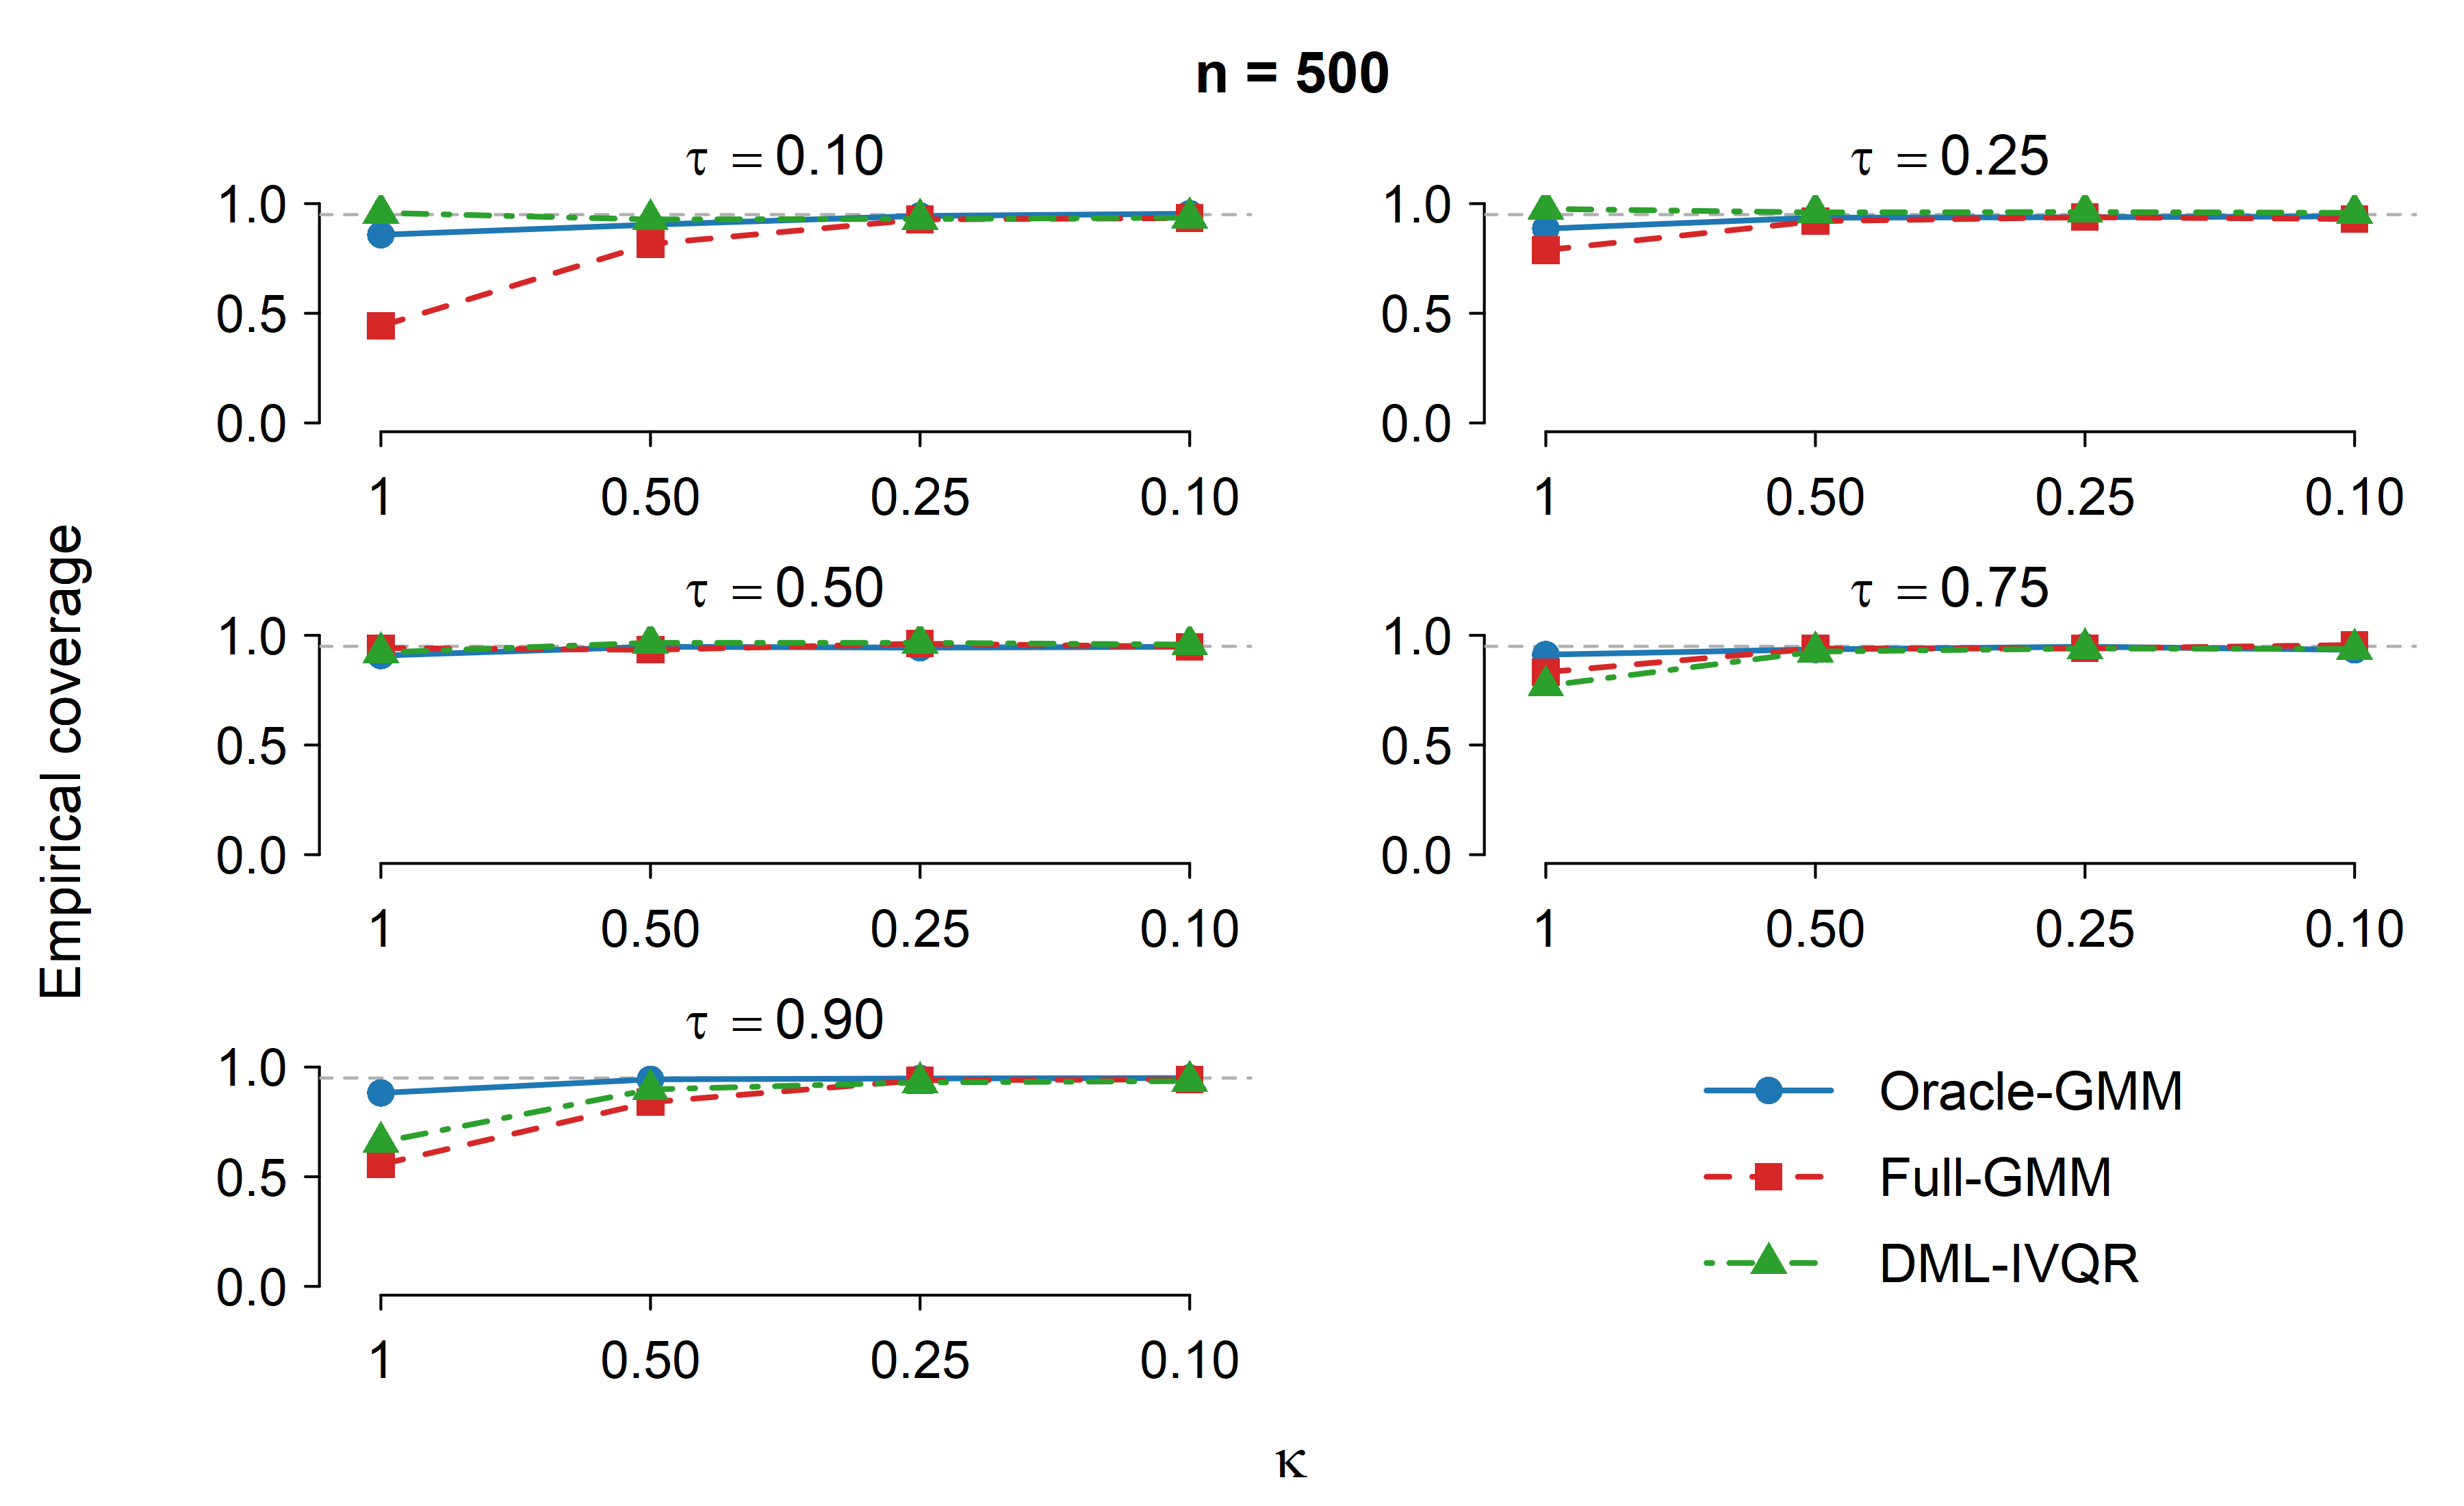
\includegraphics[width=\textwidth]{figures/generated/coverage_n500_thesis.png}
  \par\smallskip (a) $n=500$
  \par\medskip
  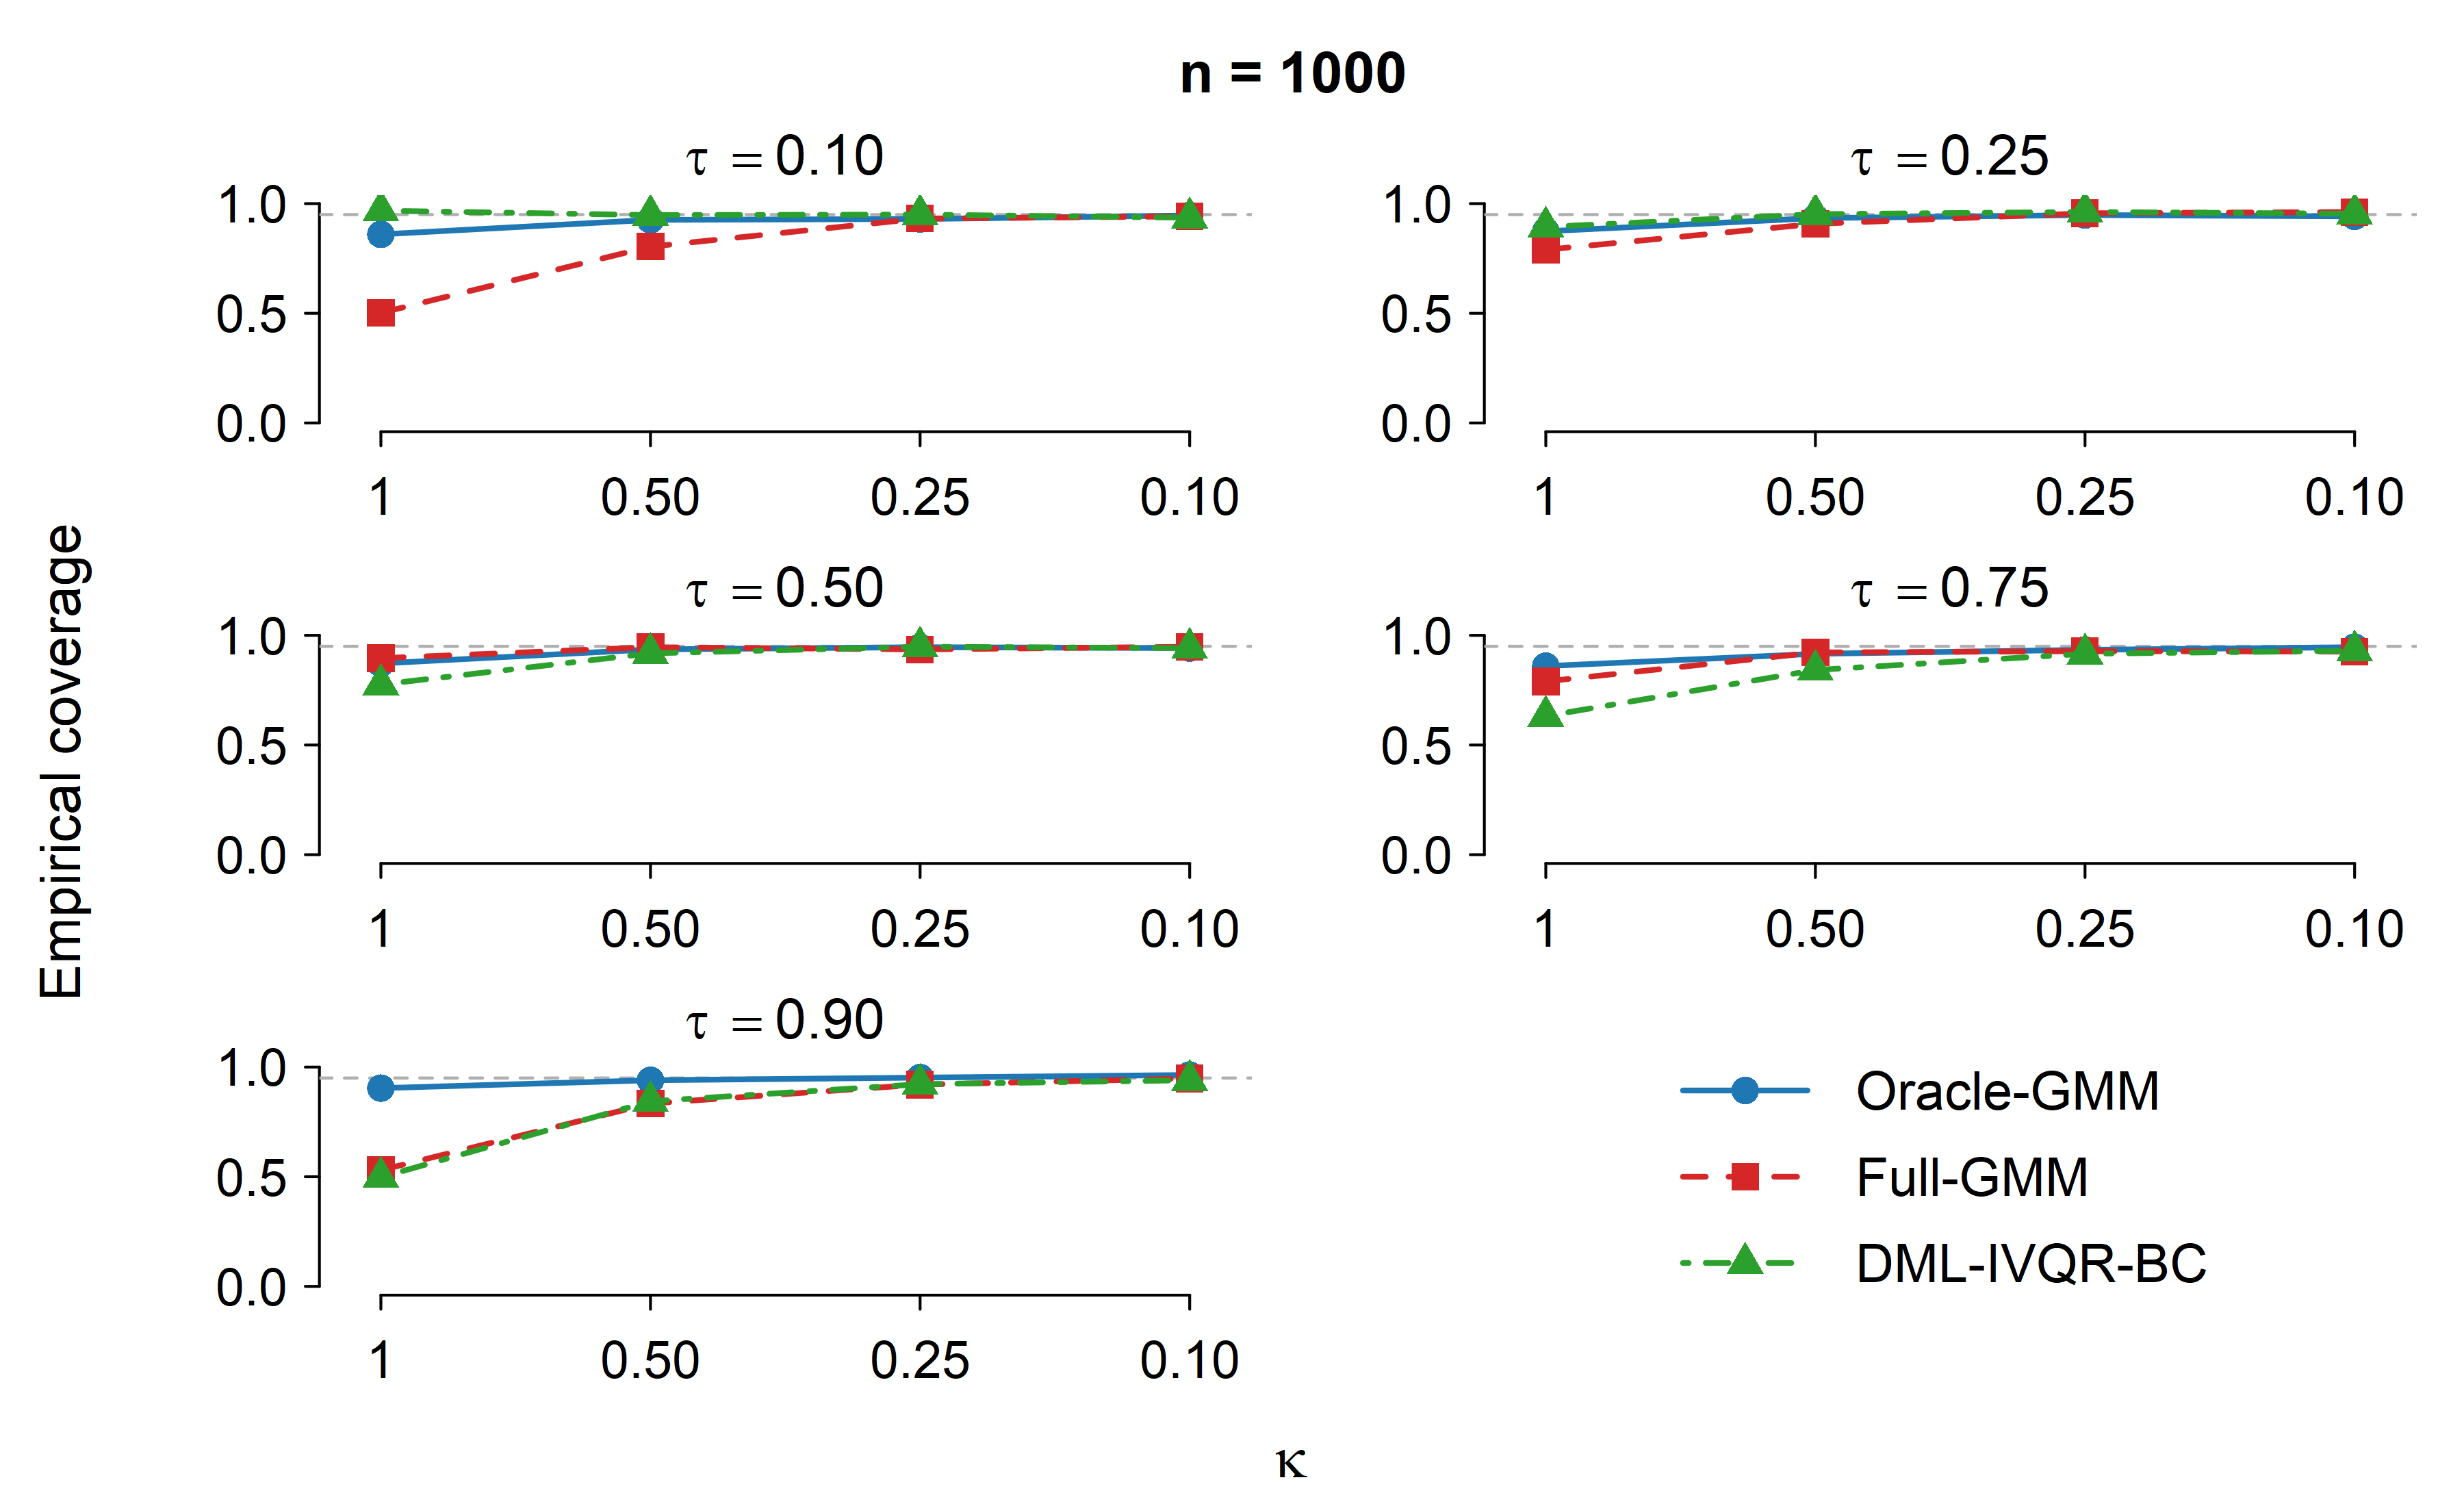
\includegraphics[width=\textwidth]{figures/generated/coverage_n1000_thesis.png}
  \par\smallskip (b) $n=1000$
  \caption{Empirical coverage across instrument-strength designs.}
  \label{fig:coverage-main}
\end{figure}


Because each reported coverage rate is based on $R=500$ Monte Carlo replications, the simulation itself introduces sampling uncertainty. For an estimated rejection or coverage probability $\widehat p$, the Monte Carlo standard error is
\[
\operatorname{MCSE}(\widehat p)
=
\sqrt{\frac{\widehat p(1-\widehat p)}{R}}.
\]
With $R=500$, the largest possible MCSE is approximately $0.022$, attained near $\widehat p=0.5$; at the nominal coverage probability $0.95$, the corresponding MCSE is approximately $0.010$. Consequently, very small differences between nearby coverage rates should not be given substantive weight. The large deviations emphasized here are materially larger than Monte Carlo uncertainty: coverage values around $0.50$, $0.63$, or $0.86$, for example, remain far from the nominal $0.95$ benchmark relative to their simulation standard errors.

Distortions occur even at $\kappa=1$ and vary substantially by estimator and quantile. For $n=1000$, Full coverage is $0.502$ at $\tau=0.10$ and $0.530$ at $\tau=0.90$. DML coverage is $0.632$ at $\tau=0.75$ and $0.498$ at $\tau=0.90$, but $0.968$ at $\tau=0.10$. Oracle coverage is $0.860$ at both $\tau=0.10$ and $\tau=0.75$, showing that high-dimensional nuisance estimation is not the sole explanation for undercoverage.

As relevance becomes very weak, the test may reject few candidates, retaining the truth frequently while accepted sets cover most of the primary domain. Such high coverage measures calibration and can coexist with very low informativeness and power.

\subsection{Confidence-Set Informativeness and Power}

Figure~\ref{fig:accepted-measure-main} shows the median grid-based accepted-set measure within $A_0=[-1,3]$. Panels (a) and (b) report $n=500$ and $n=1000$, respectively, allowing comparison across sample sizes for the same quantiles and estimators. The plotted quantity measures acceptance inside the four-unit primary domain, not unrestricted confidence-region length.

% Prepared for later insertion; the legend in panel (b) applies to both panels.
\begin{figure}[p]
  \centering
  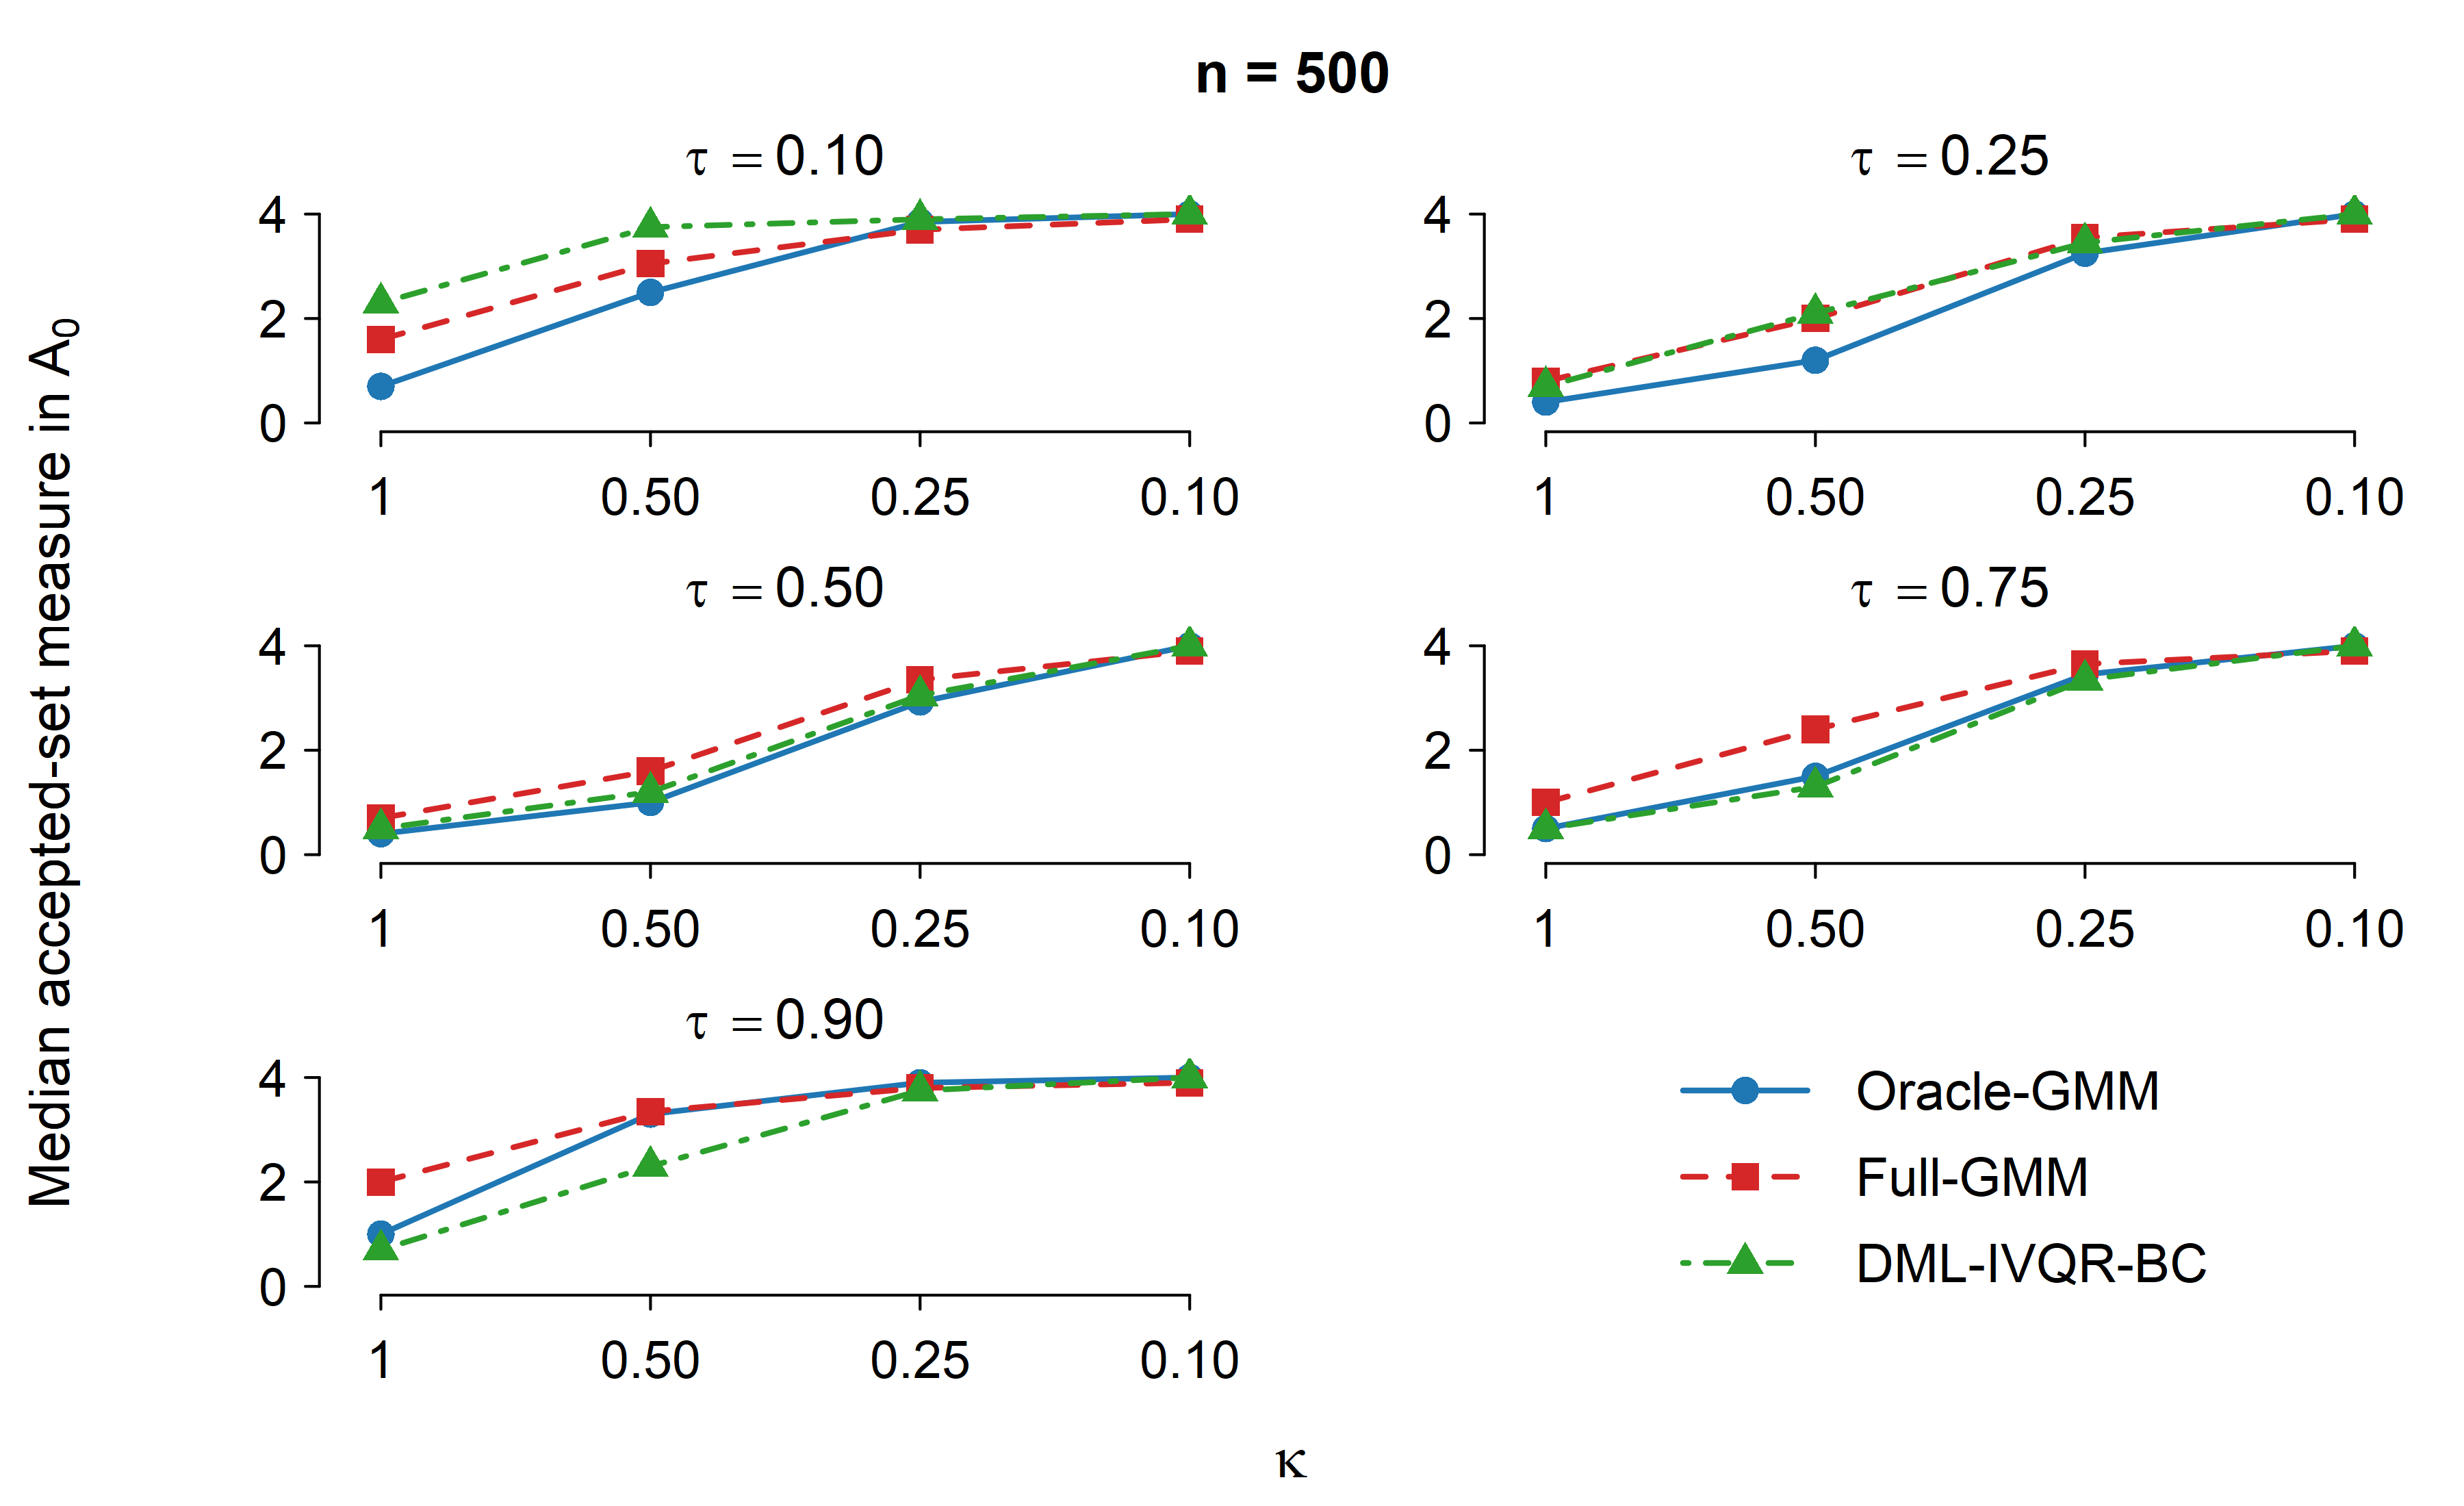
\includegraphics[width=\textwidth]{figures/generated/accepted_measure_n500_thesis.png}
  \par\smallskip (a) $n=500$
  \par\medskip
  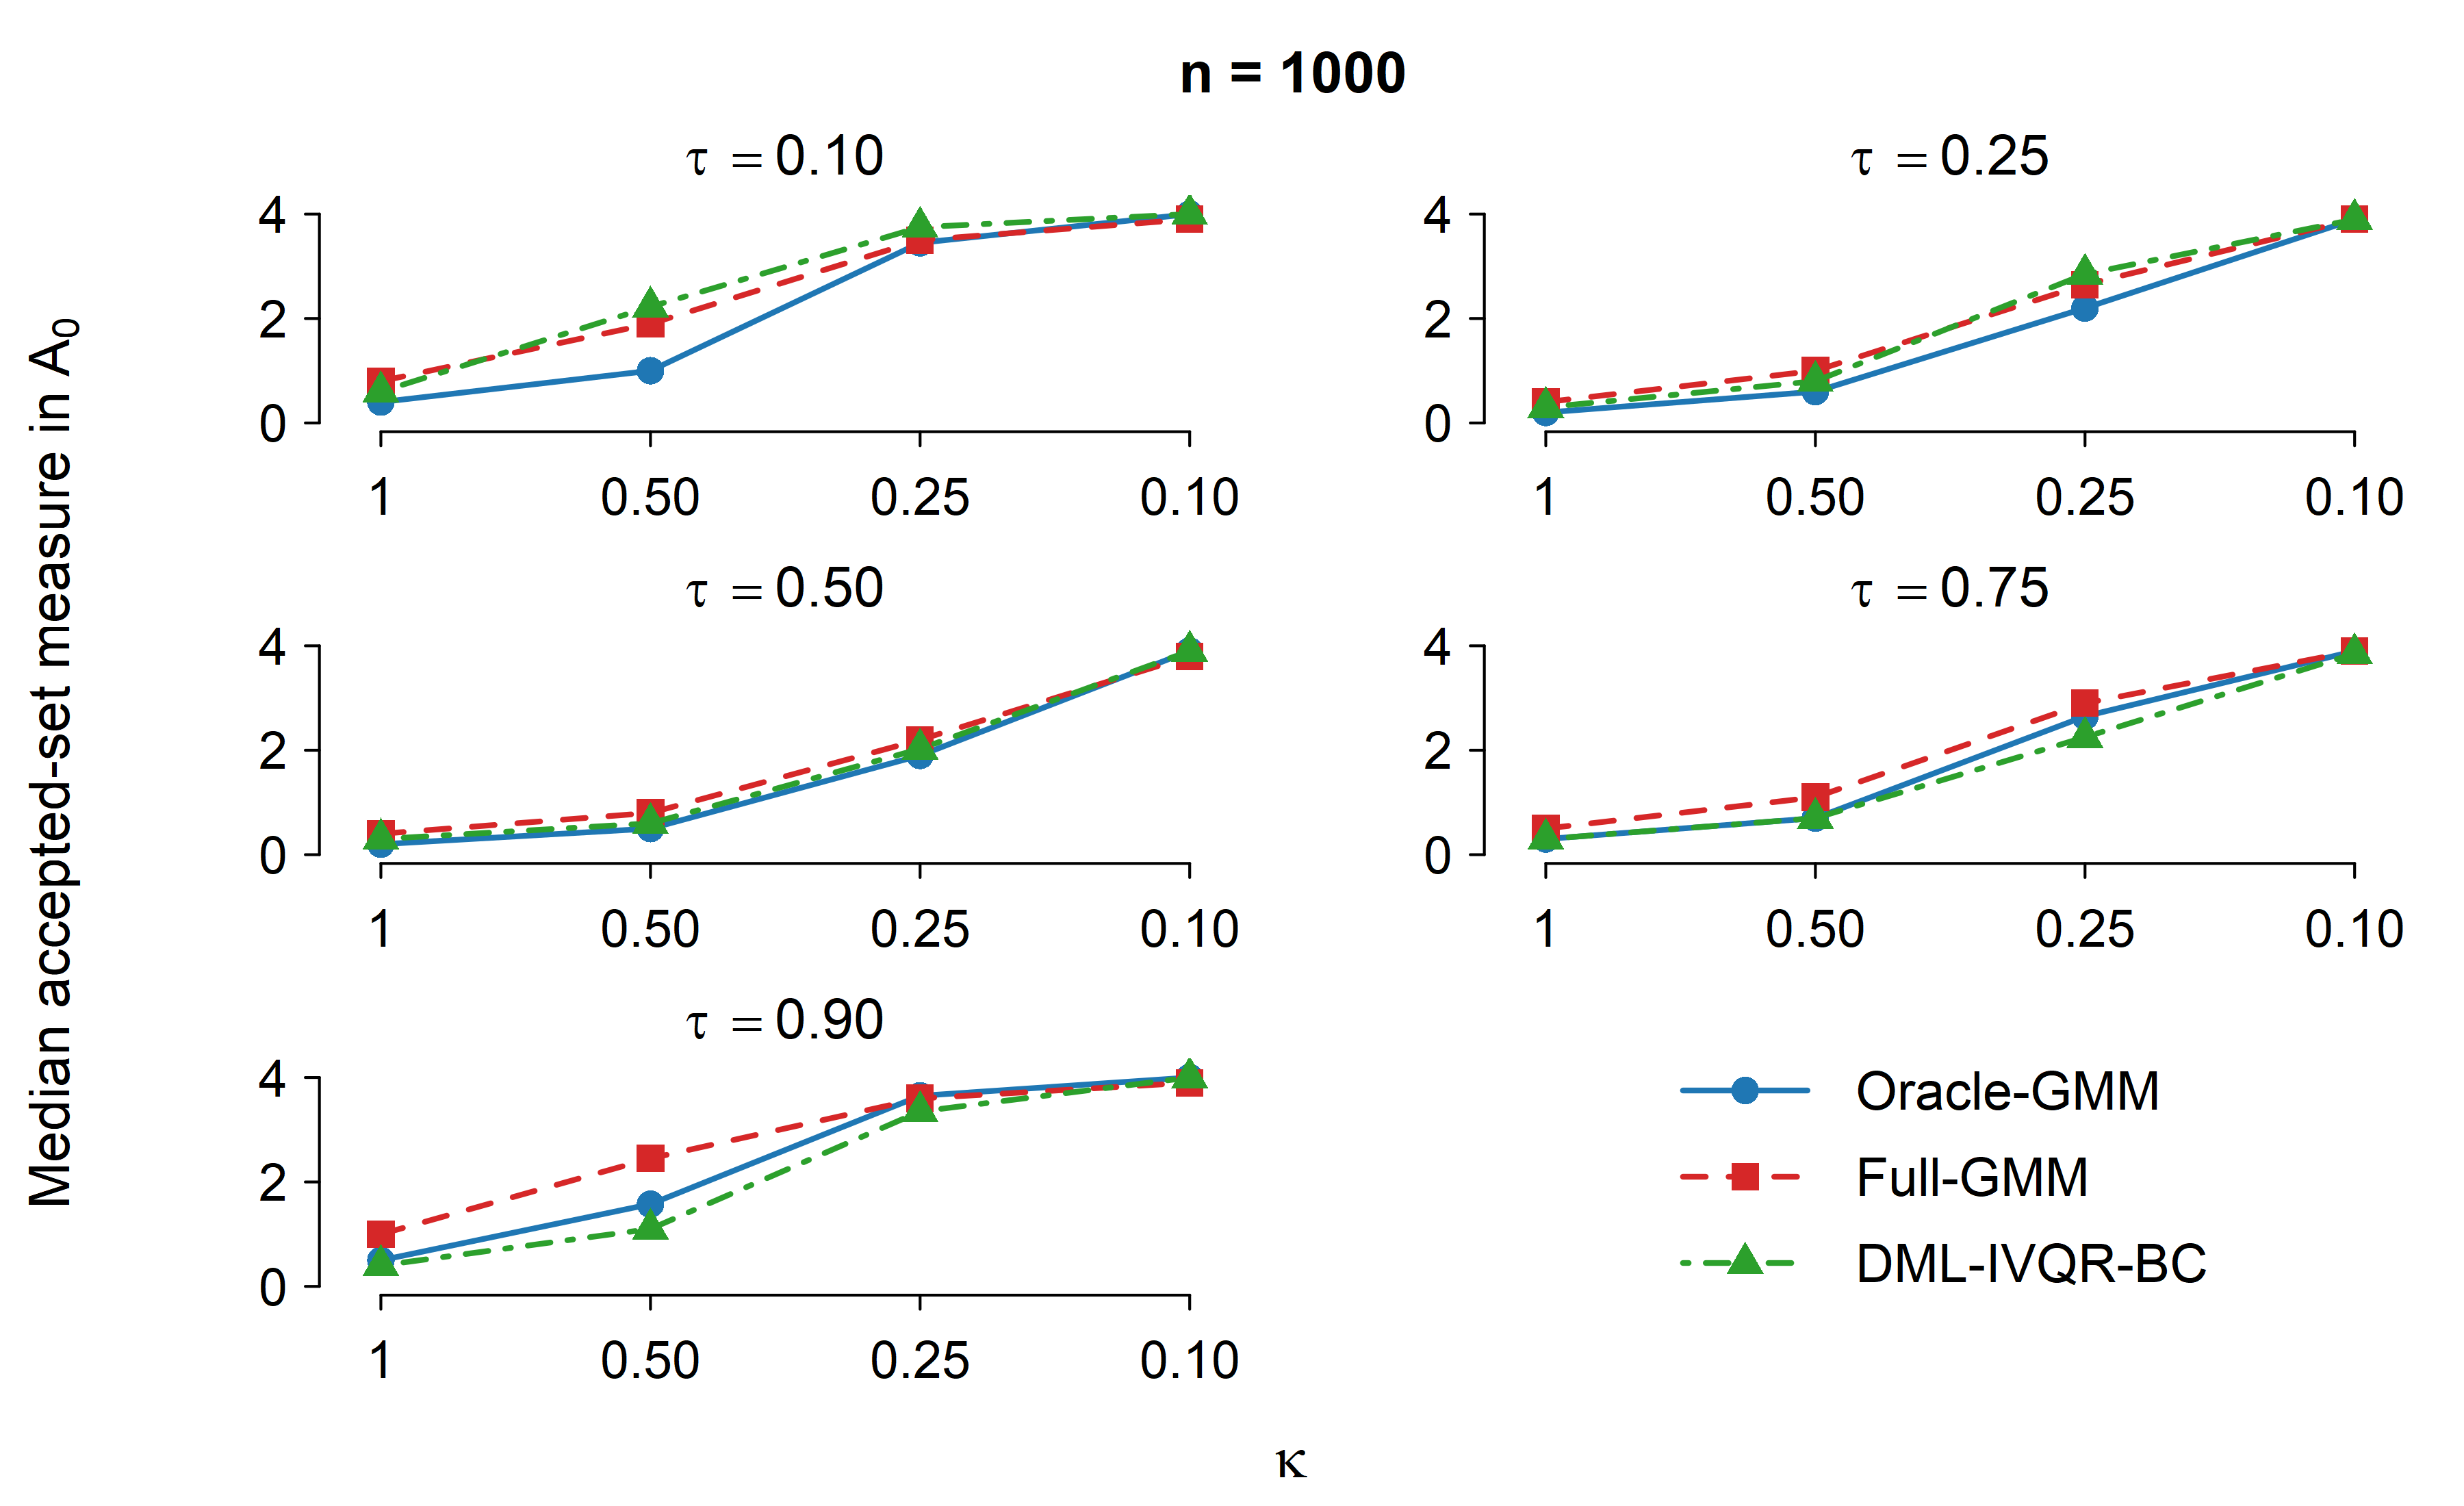
\includegraphics[width=\textwidth]{figures/generated/accepted_measure_n1000_thesis.png}
  \par\smallskip (b) $n=1000$
  \caption{Grid-based accepted-set measure within the primary computational domain $A_0=[-1,3]$.}
  \label{fig:accepted-measure-main}
\end{figure}


The measure rises strongly as $\kappa$ falls, and at $\kappa=0.10$ accepted sets often occupy nearly the whole primary domain. For $n=1000$ and $\tau=0.50$, the Oracle, Full, and DML medians rise respectively from $0.200$, $0.400$, and $0.300$ at $\kappa=1$ to $3.900$, $3.800$, and $3.900$ at $\kappa=0.10$. Increasing $n$ generally improves localization, but does not solve the weakest-relevance case. The accepted-set measure is deliberately defined on the fixed primary domain $A_0=[-1,3]$; the separate domain diagnostic is reserved for the Appendix.

Figure~\ref{fig:power-main} reports rejection probabilities under moderate false alternatives for $n=1000$: panel (a) uses $\Delta=-0.50$ and panel (b) uses $\Delta=+0.50$. Rejection probabilities fall strongly as $\kappa$ decreases, so false candidate treatment effects survive more frequently.

% Prepared for later insertion; the legend in panel (b) applies to both panels.
\begin{figure}[p]
  \centering
  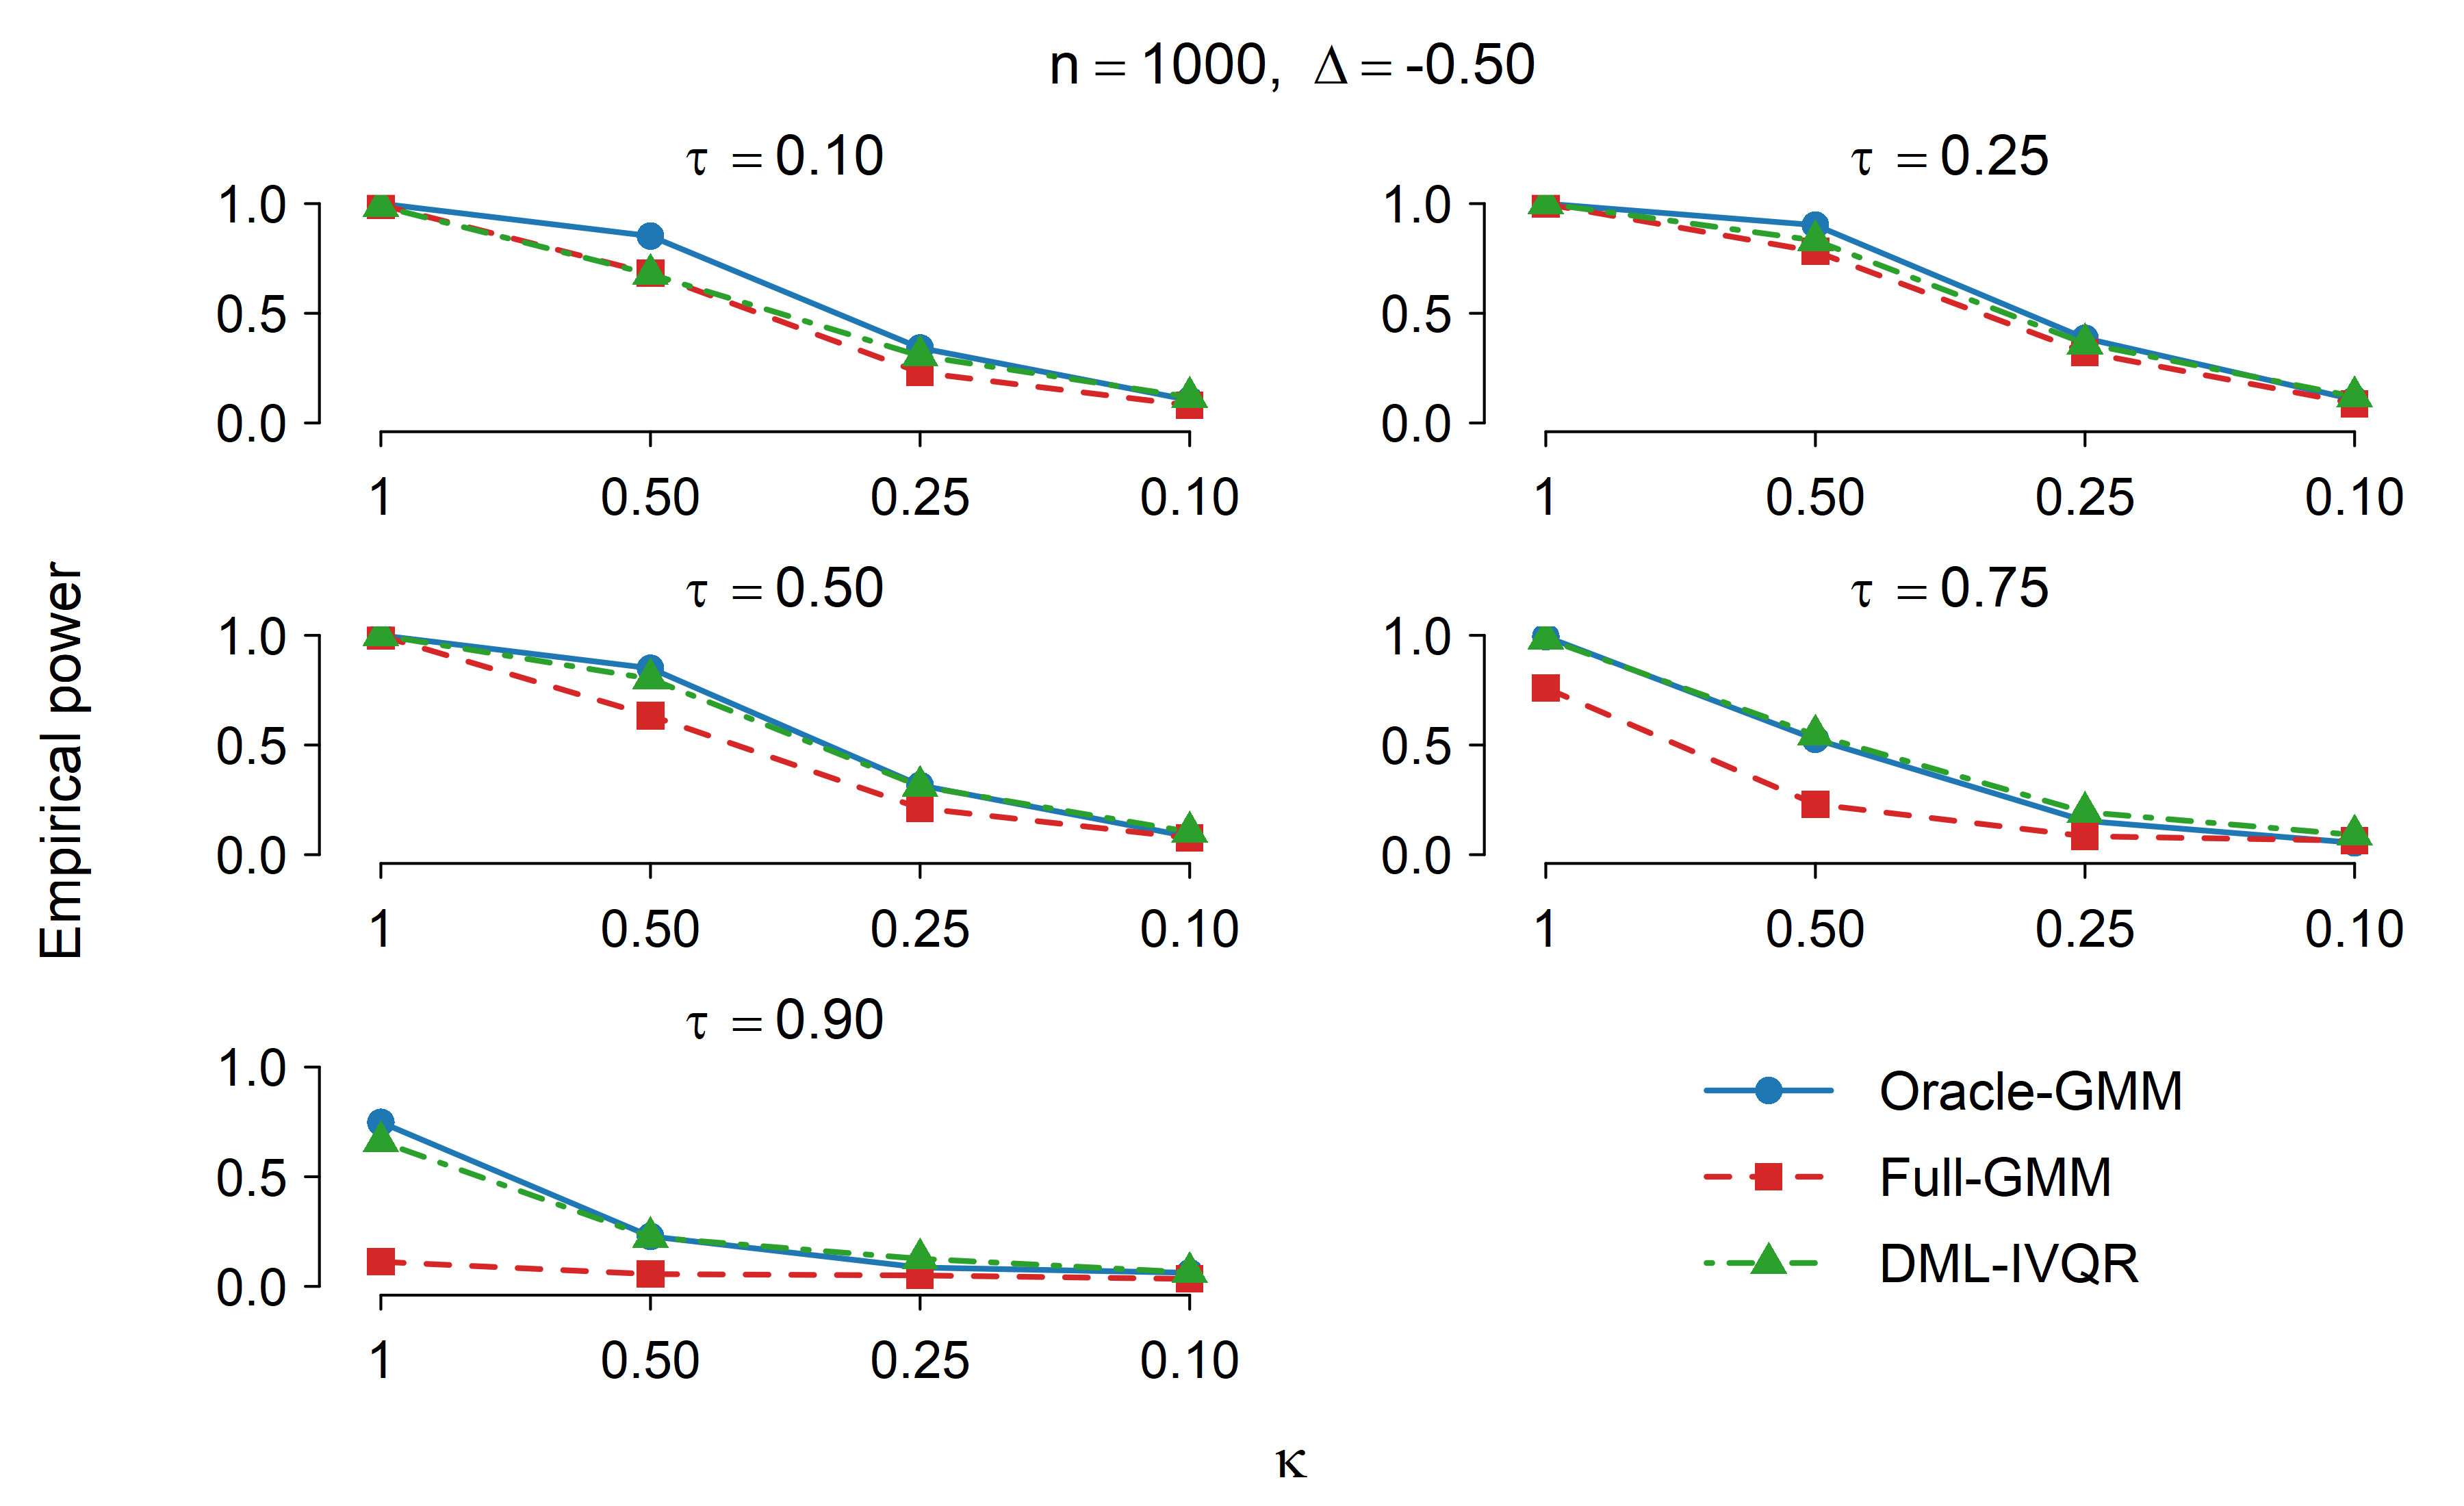
\includegraphics[width=\textwidth]{figures/generated/power_minus050_n1000_thesis.png}
  \par\smallskip (a) $\Delta=-0.50$
  \par\medskip
  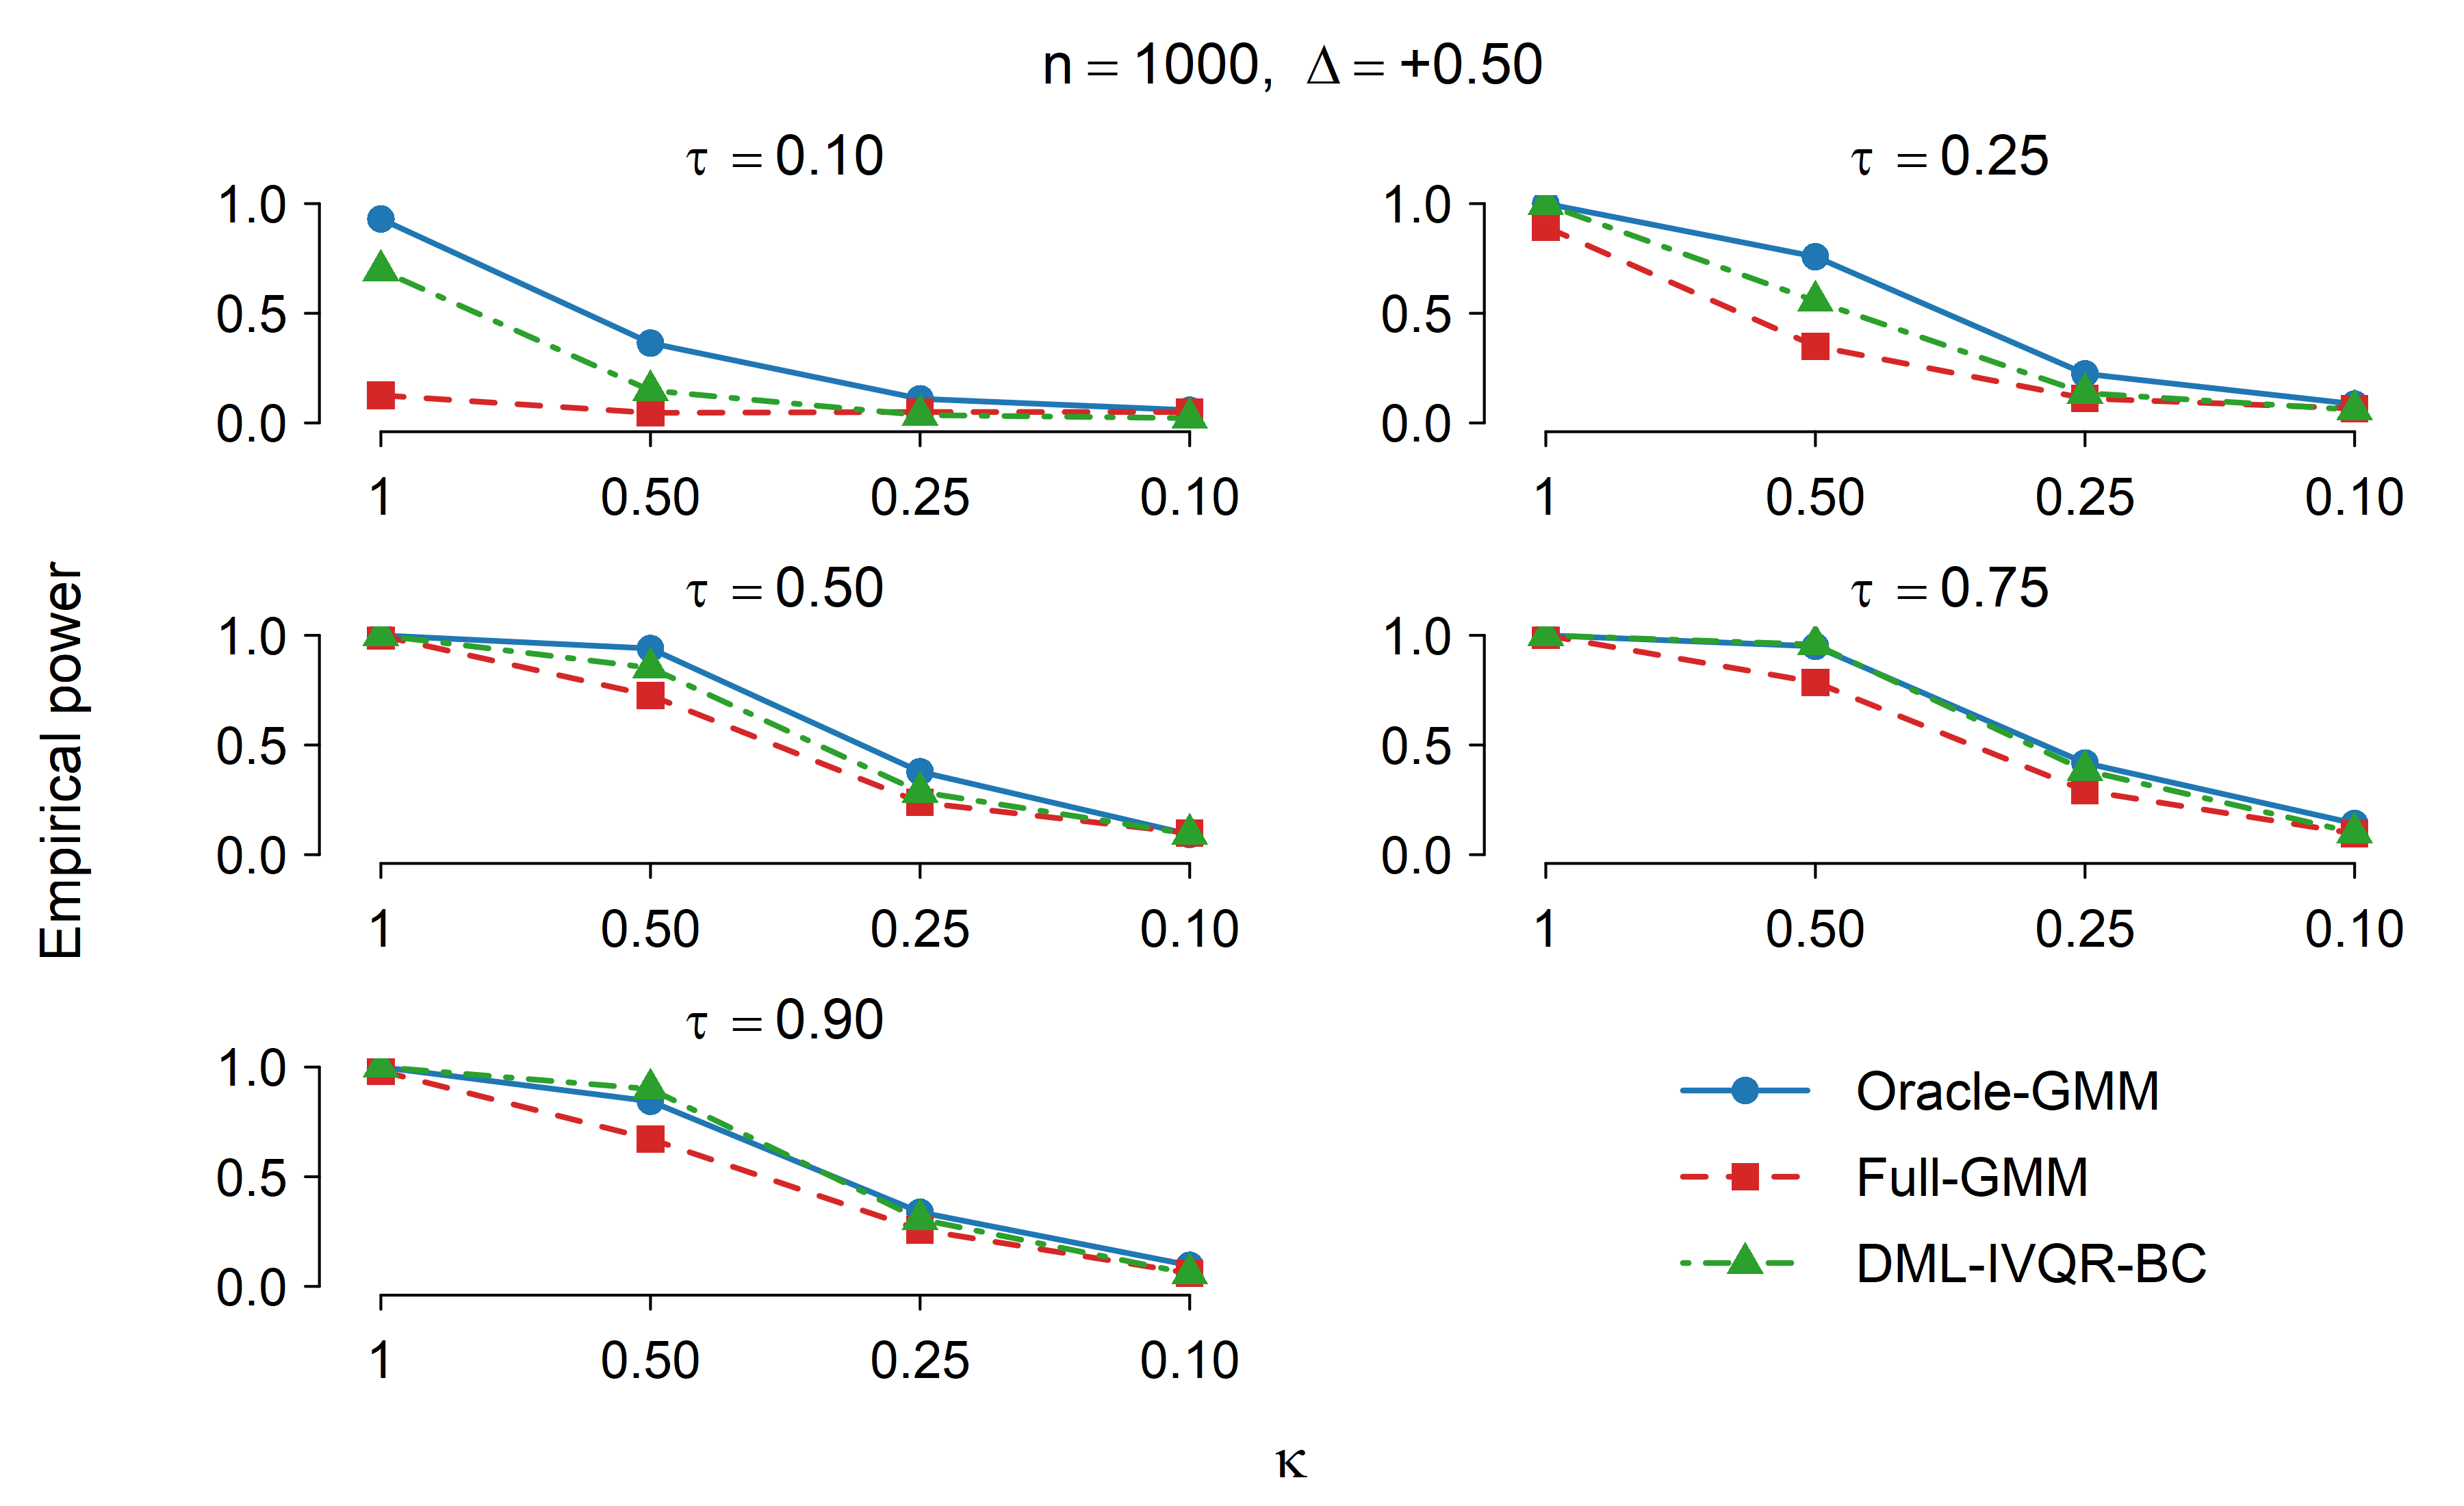
\includegraphics[width=\textwidth]{figures/generated/power_plus050_n1000_thesis.png}
  \par\smallskip (b) $\Delta=+0.50$
  \caption{Rejection probability under moderate false alternatives, $n=1000$.}
  \label{fig:power-main}
\end{figure}


At $\tau=0.50$ and $\Delta=-0.50$, power falls from $1.000$ to $0.082$ for Oracle, from $0.998$ to $0.076$ for Full, and from $1.000$ to $0.104$ for DML as $\kappa$ falls from $1$ to $0.10$. At the positive alternative, the corresponding weakest-relevance probabilities are $0.092$, $0.098$, and $0.094$. Positive and negative alternatives need not behave symmetrically because the candidate-specific moments can distinguish equally sized departures differently across directions. The accepted-set and power results are two complementary manifestations of declining informativeness.

\subsection{Quantile Heterogeneity and Estimator Comparison}

Taken together, Table~\ref{tab:main-performance} and Figures~\ref{fig:coverage-main}--\ref{fig:power-main} show that weakening relevance worsens performance across quantiles, although the magnitude differs. Tail quantiles often display larger estimation errors or more severe calibration problems, but there is no universal ordering between the center and tails or between the two tails.

Oracle generally provides the strongest benchmark, yet deteriorates sharply as relevance weakens. DML often improves on Full, but does not dominate it in every cell or reproduce Oracle uniformly. These differences cannot be attributed solely to regularization because the estimators also use different residualization conventions.

Weaker excluded-instrument relevance raises point-estimation error, reduces the ability to reject false candidate values, and expands the set of accepted treatment-effect values. These effects occur for Oracle, Full, and DML-IVQR and vary across quantiles. Regularized nuisance estimation can improve performance relative to the unregularized high-dimensional benchmark in some cells, but it cannot replace missing instrument information.

\clearpage
